\section{Données}
\label{sec:data}
Cette section détaille la collecte, la sélection et l'analyse des données utilisées pour examiner l'impact de l'introduction de la taxe CO2 en 2008 en Suisse sur les émissions de gaz à effet de serre. Pour renforcer la robustesse de notre analyse, nous avons utilisé deux approches complémentaires : l'analyse de différence en différences (DiD) avec l'Autriche comme pays de contrôle, et la méthode de contrôle synthétique (SCM) l'Aautriche, le Luxembourg et la Hollande.


\subsection{Données sélectionnées}
\label{subsec:data_selection}


Les données ont été collectées sur le site de l'Organisation de Coopération et de Développement Économiques (OCDE) ainsi que sur le site Our World in Data, des sources fiables et reconnues pour les statistiques économiques, énergétiques et environnementales.

\textbf{Variables Clés}

Les variables sélectionnées pour l'analyse sont cruciales pour comprendre l'impact de la taxe CO2 sur les émissions de gaz à effet de serre. Ces variables ont été choisies en raison de leur pertinence dans les études environnementales et économiques.  Elles comprennent :

\begin{itemize}[itemsep=-0.5em]

    \item[] \textbf{Émissions de CO2 par habitant} (tonnes) (OCDE) \supercite{greenhouse}: 
    \item[] Mesure des émissions de CO2 par individu, un indicateur clé de la performance environnementale.

    \item[] \textbf{Population} (en millions) (OCDE) \supercite{oecd_population}: 
    \item[] Mesure essentielle pour comparer l'impact démographique sur les émissions de CO2.
    \item[] \textbf{Transport passager par rail } (passager-kilomètres, millions) (OCDE)\supercite{oecd2023} : 
    \item[] Indicateur de l'activité de transport, directement lié aux émissions de CO2.
    
    \item[] \textbf{Nombre de véhicules } (par milliers d'habitants) (OCDE) \supercite{oecd_transport} : 
    \item[] Inclut les véhicules privés et commerciaux, une source majeure d'émissions de CO2.
    
    \item[] \textbf{Variation du PIB par habitant (\%)} (OCDE) \supercite{gdp} : 
    \item[] Indicateur économique clé reflétant la croissance et la prospérité économique, influençant potentiellement les émissions de CO2.
    
    
    \item[] \textbf{Consommation énergétique} (en MWh/habitant) (Our World in Data) \supercite{energy} : 
    \item[] Indicateur de la dépendance énergétique du pays, bien que cette variable ait été exclue de l'analyse finale en raison de données limitées.
\end{itemize}



En plus de déterminer une période d'observation adéquate il est essentiel de choisir un pays de contrôle approprié pour notre analyse DiD afin de garantir la robustesse et la validité des résultats obtenus.

\subsubsection{Période d'observation}
\label{subsec:observation_period}

Nous avons choisi une période d'observation allant de 1994 à 2018 afin de maximiser l'étendue des données disponibles avant et après l'introduction de la taxe CO2. La période post-traitement a été limitée à 2018 pour éviter les perturbations causées par la pandémie de COVID-19, qui a eu un impact significatif sur les émissions de CO2.

\textbf{Justification de l'exclusion des données post-2018}


L'exclusion des données après 2018 est basée sur le fait que la pandémie de COVID-19 a créé des perturbations majeures dans les émissions de CO2 en raison de changements drastiques dans les comportements économiques et sociaux, comme les confinements et la réduction significative des activités industrielles et de transport. Intégrer ces données pourrait introduire des biais importants et fausser l'analyse de l'impact de la taxe CO2.

\subsection{Sélection du pays de contrôle}
\label{subsec:control}

Afin de sélectionner le meilleur pays de contrôle pour l'analyse DiD (Différence en Différences), nous avons évalué plusieurs pays candidats en utilisant une méthode visuelle basée sur les ajustements de courbes et la comparaison des écarts avec la Suisse. Les pays candidats initialement évalués étaient (entre parenthèse la date d'introduction de la taxe CO$_2$ du pays): l'Autriche (2022), la France (2014), l'Allemagne (2021), l'Espagne (2014), l'Irlande (2010), le Portugal (2015), le Luxembourg (2021), et les Pays-Bas (2021).

\textbf{Procédure d'élimination :}

\begin{enumerate}
    \item Comparaison des variables explicatives : nous avons comparé visuellement les variables explicatives de chaque pays candidat avec celles de la Suisse en utilisant des graphiques d'ajustement de courbes. Les pays dont les variables différaient significativement ont été éliminés.
\item Dates d'introduction de la taxe CO2 : nous avons considéré un avantage pour les pays avec les dates les plus distantes pour maximiser l'étendue des observations post-traitement.
\end{enumerate}

\textbf{Visualisation de la comparaison :}

Les graphiques ci-dessous montrent la comparaison des variables explicatives entre la Suisse et les pays candidats. Chaque graphique présente les tendances des variables clés (population, PIB par habitant, transport passager par rail, nombre de véhicules) pour chaque pays candidat par rapport à la Suisse. Les éliminations des pays candidats sont également indiquées à chaque étape.

\vspace{1cm}

        \begin{figure}[H]
\textbf{Figure {$\ref{fig:trend_transport}$}} : 
Le graphique ci-dessous compare les variables "transports par rail" entre la Suisse et les pays candidats. Les écarts significatifs observés pour certains pays ont conduit à leur élimination à cette étape.
        \centering
        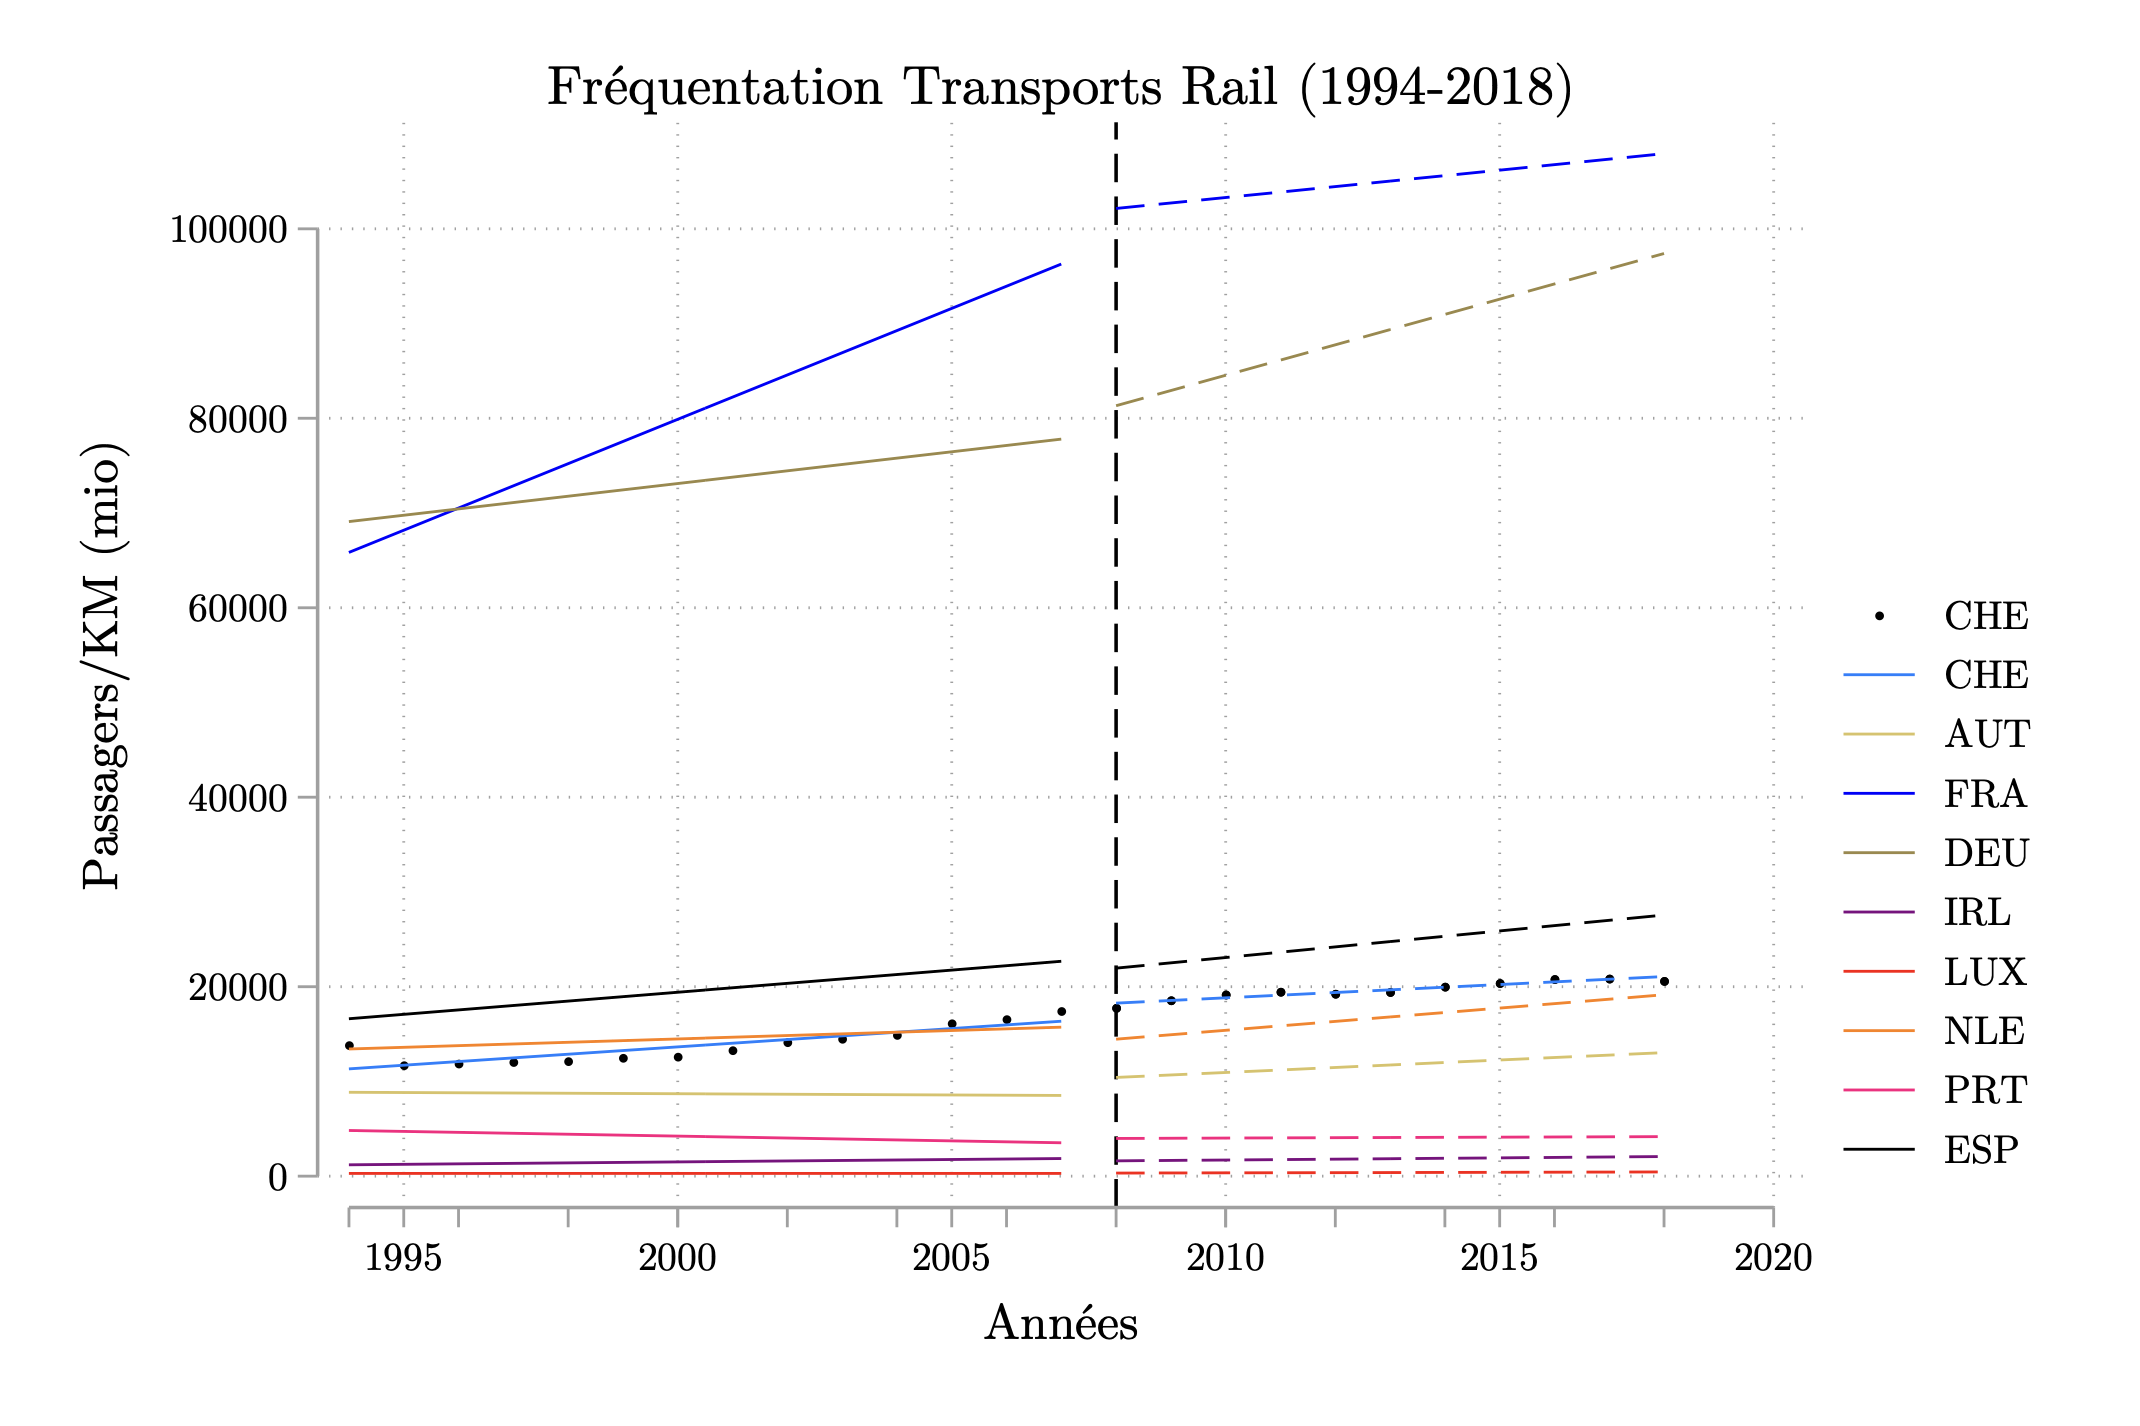
\includegraphics[width=0.6\textwidth]{Article/images/trend_transport.png}
        \caption{}
        \label{fig:trend_transport}
\begin{center}
   Élimination : France et Allemagne (écart significatif dans le transport passager par rail par rapport à la Suisse) 
\end{center}
    \end{figure}



%------------------------------------------------------------------------------------%
% \newpage 
%------------------------------------------------------------------------------------%

        \begin{figure}[H]
\textbf{Figure {$\ref{fig:trend_pop}$}} : Le graphique ci-dessous compare les variables "population" entre la Suisse et les pays candidats. Les écarts significatifs observés pour certains pays ont conduit à leur élimination à cette étape. Comparaison de la population


        \centering
        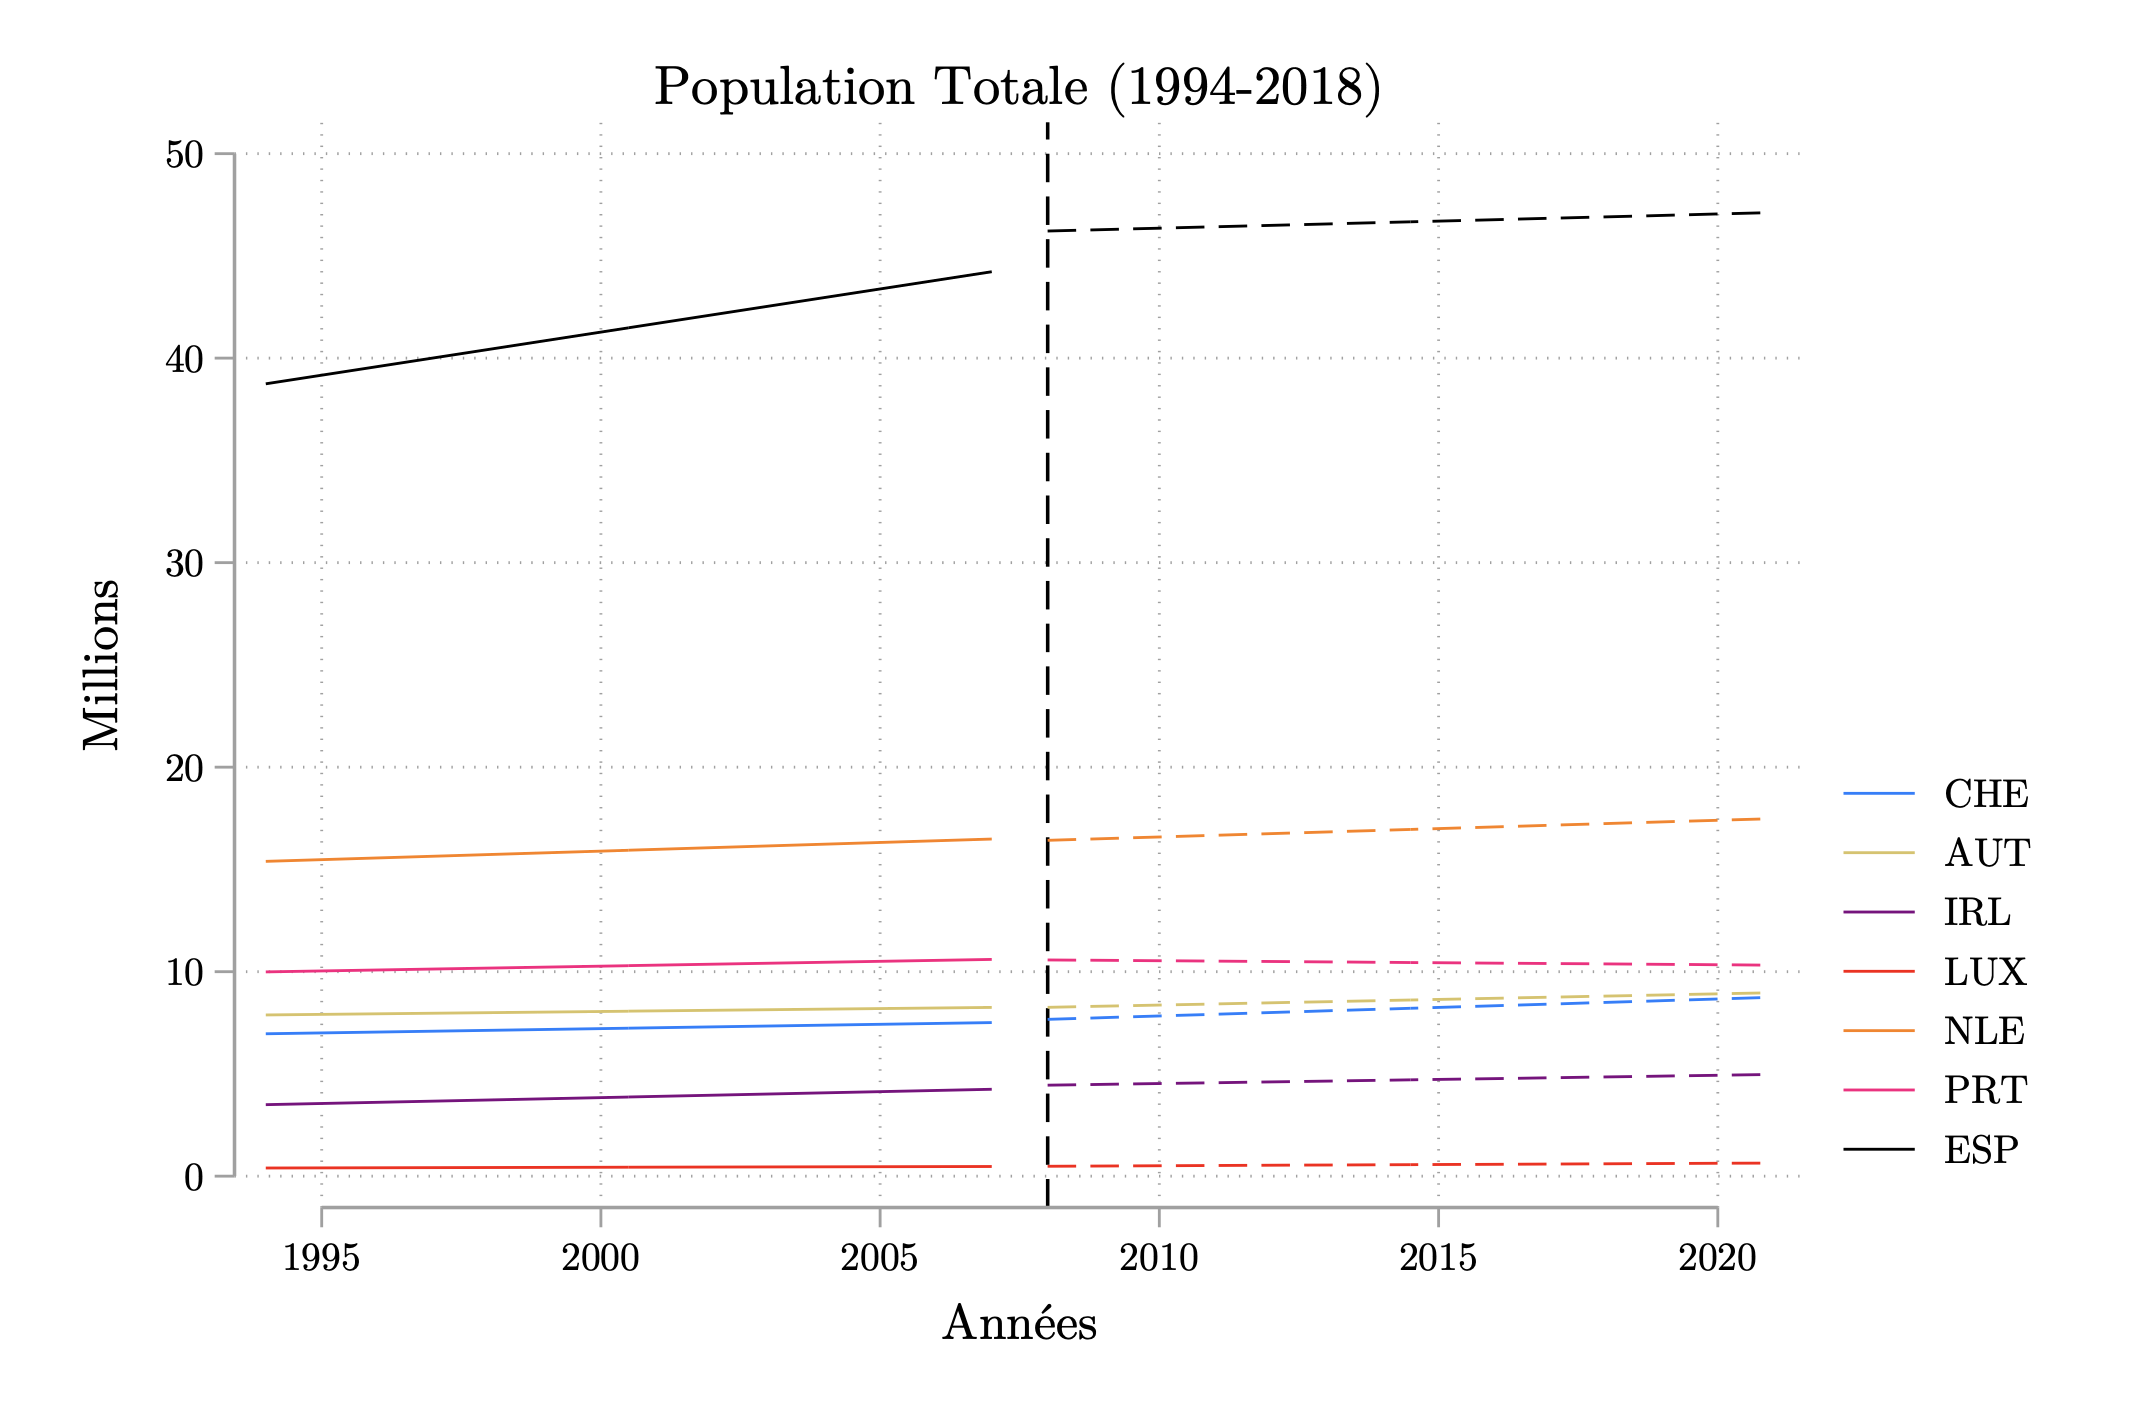
\includegraphics[width=0.6\textwidth]{Article/images/trend_population.png}
        \caption{}
        \label{fig:trend_pop}
\begin{center}
    Élimination : Espagne (écart significatif de la population par rapport à la Suisse).
\end{center}
    \end{figure}

    

\vspace{1cm}


        \begin{figure}[H]
\textbf{Figure {$\ref{fig:trend_pib}$}} : Le graphique ci-dessous compare les variables "PIB par Habitant" entre la Suisse et les pays candidats. Les écarts significatifs observés pour certains pays ont conduit à leur élimination à cette étape.


        \centering
        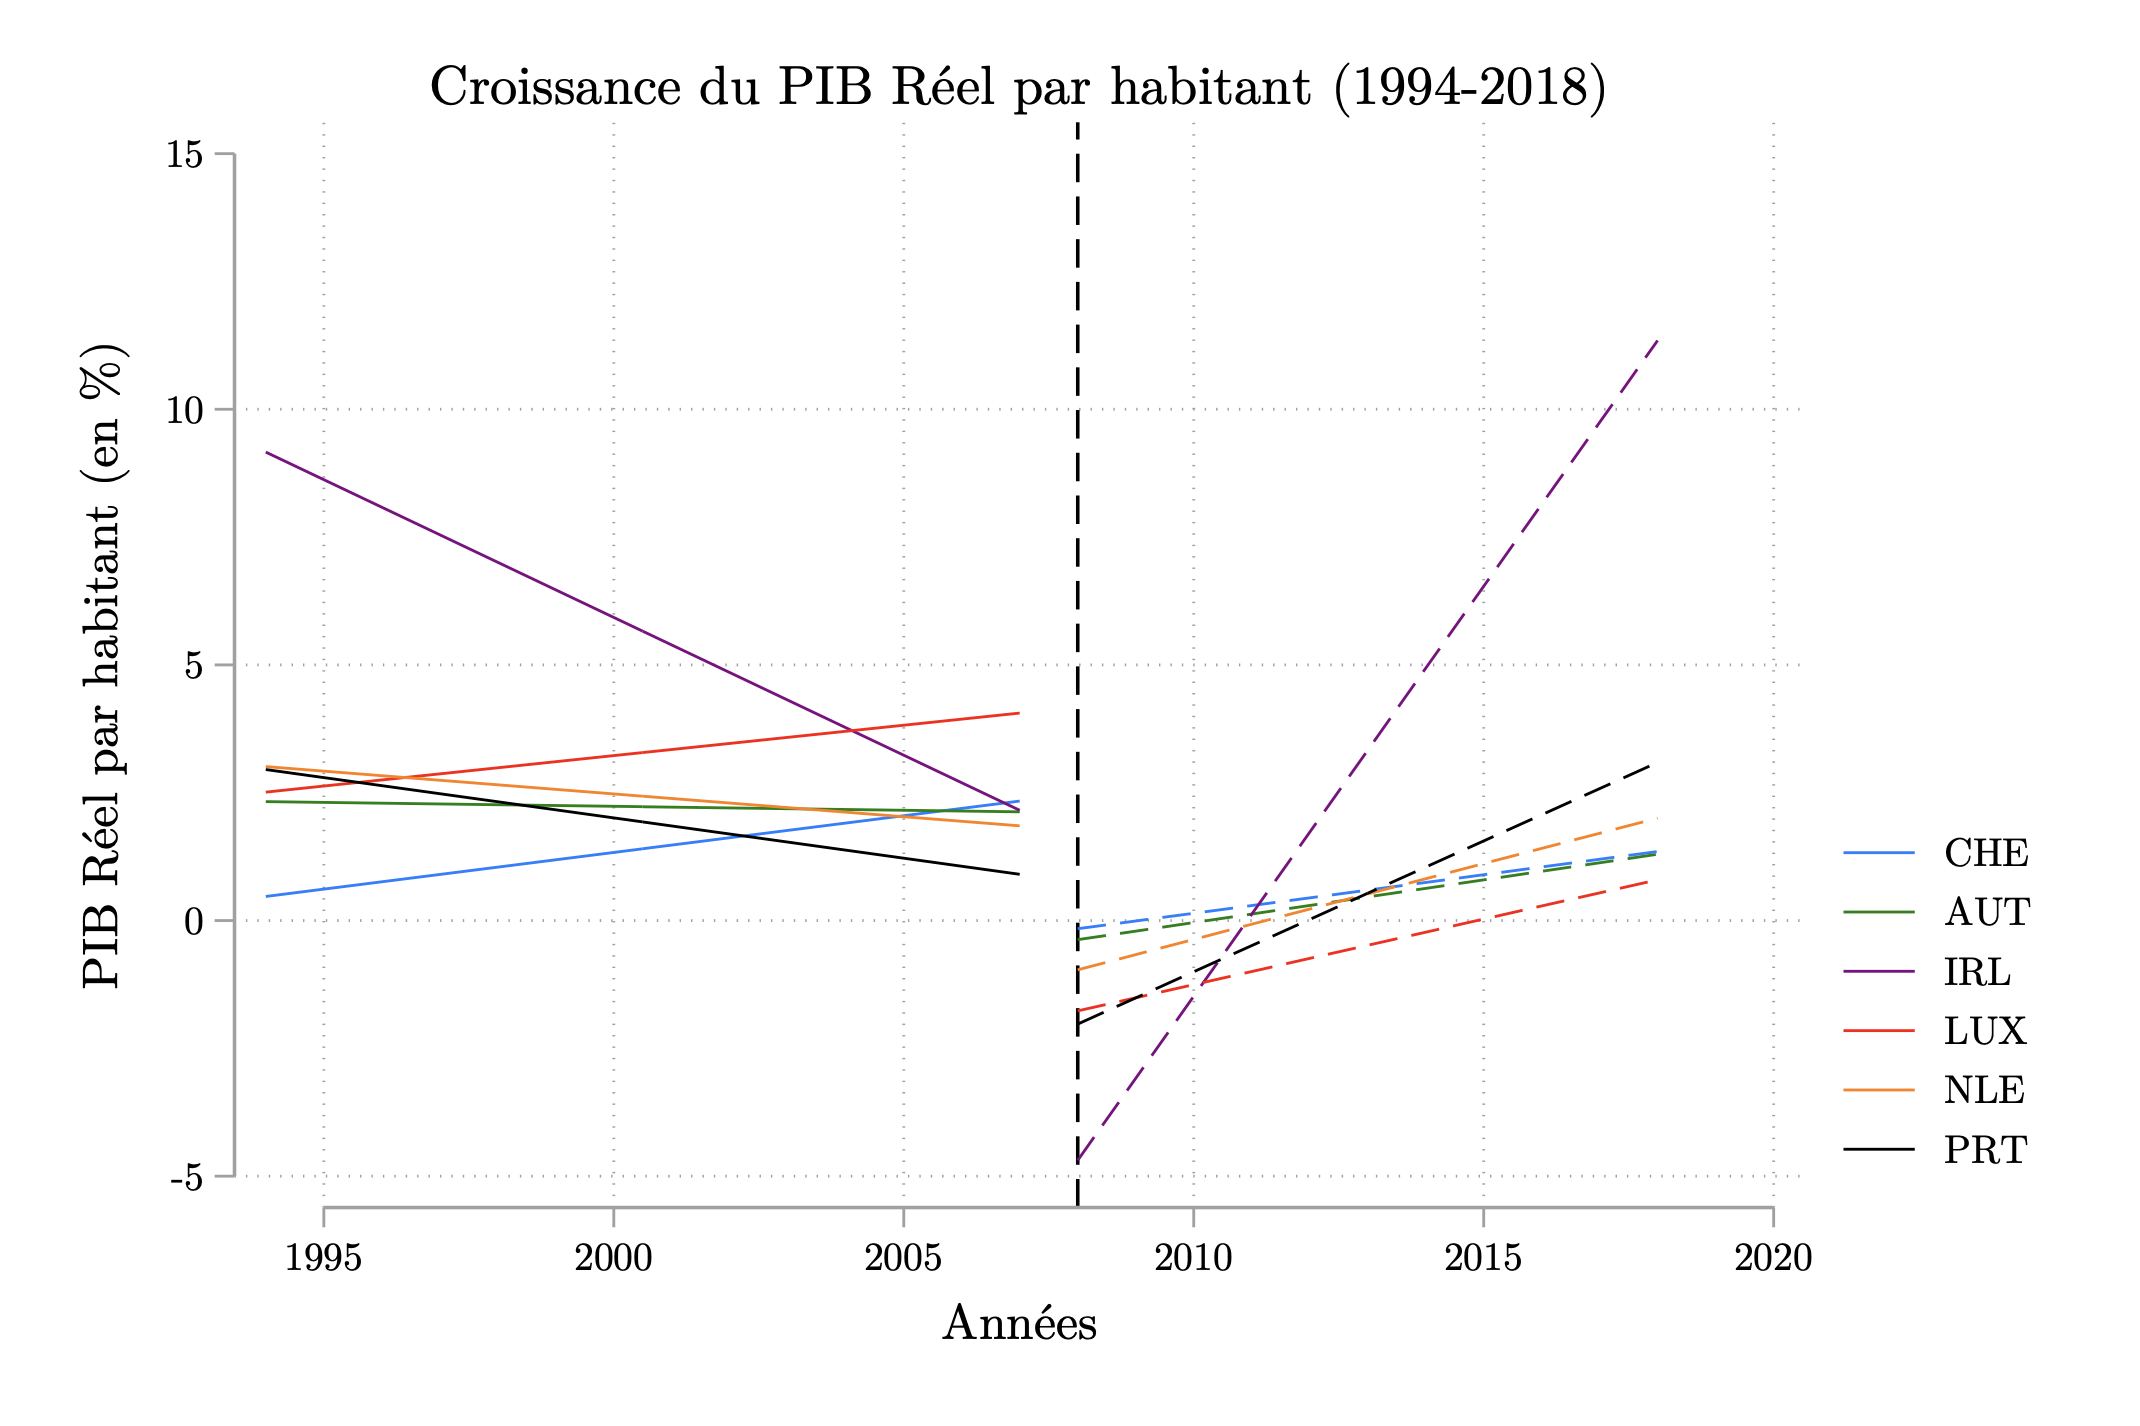
\includegraphics[width=0.6\textwidth]{Article/images/trend_pib.png}
        \caption{}
        \label{fig:trend_pib}
\begin{center}
Élimination : Irlande (écart significatif dans le PIB par habitant par rapport à la Suisse).
\end{center}
    \end{figure}

%------------------------------------------------------------------------------------%
% \newpage 
%------------------------------------------------------------------------------------%

        \begin{figure}[H]
\textbf{Figure {$\ref{fig:trend_megawats}$}} : Le graphique ci-dessous compare les variables "onsommation d'électricité" entre la Suisse et les pays candidats. Les écarts significatifs observés pour certains pays ont conduit à leur élimination à cette étape.


        \centering
        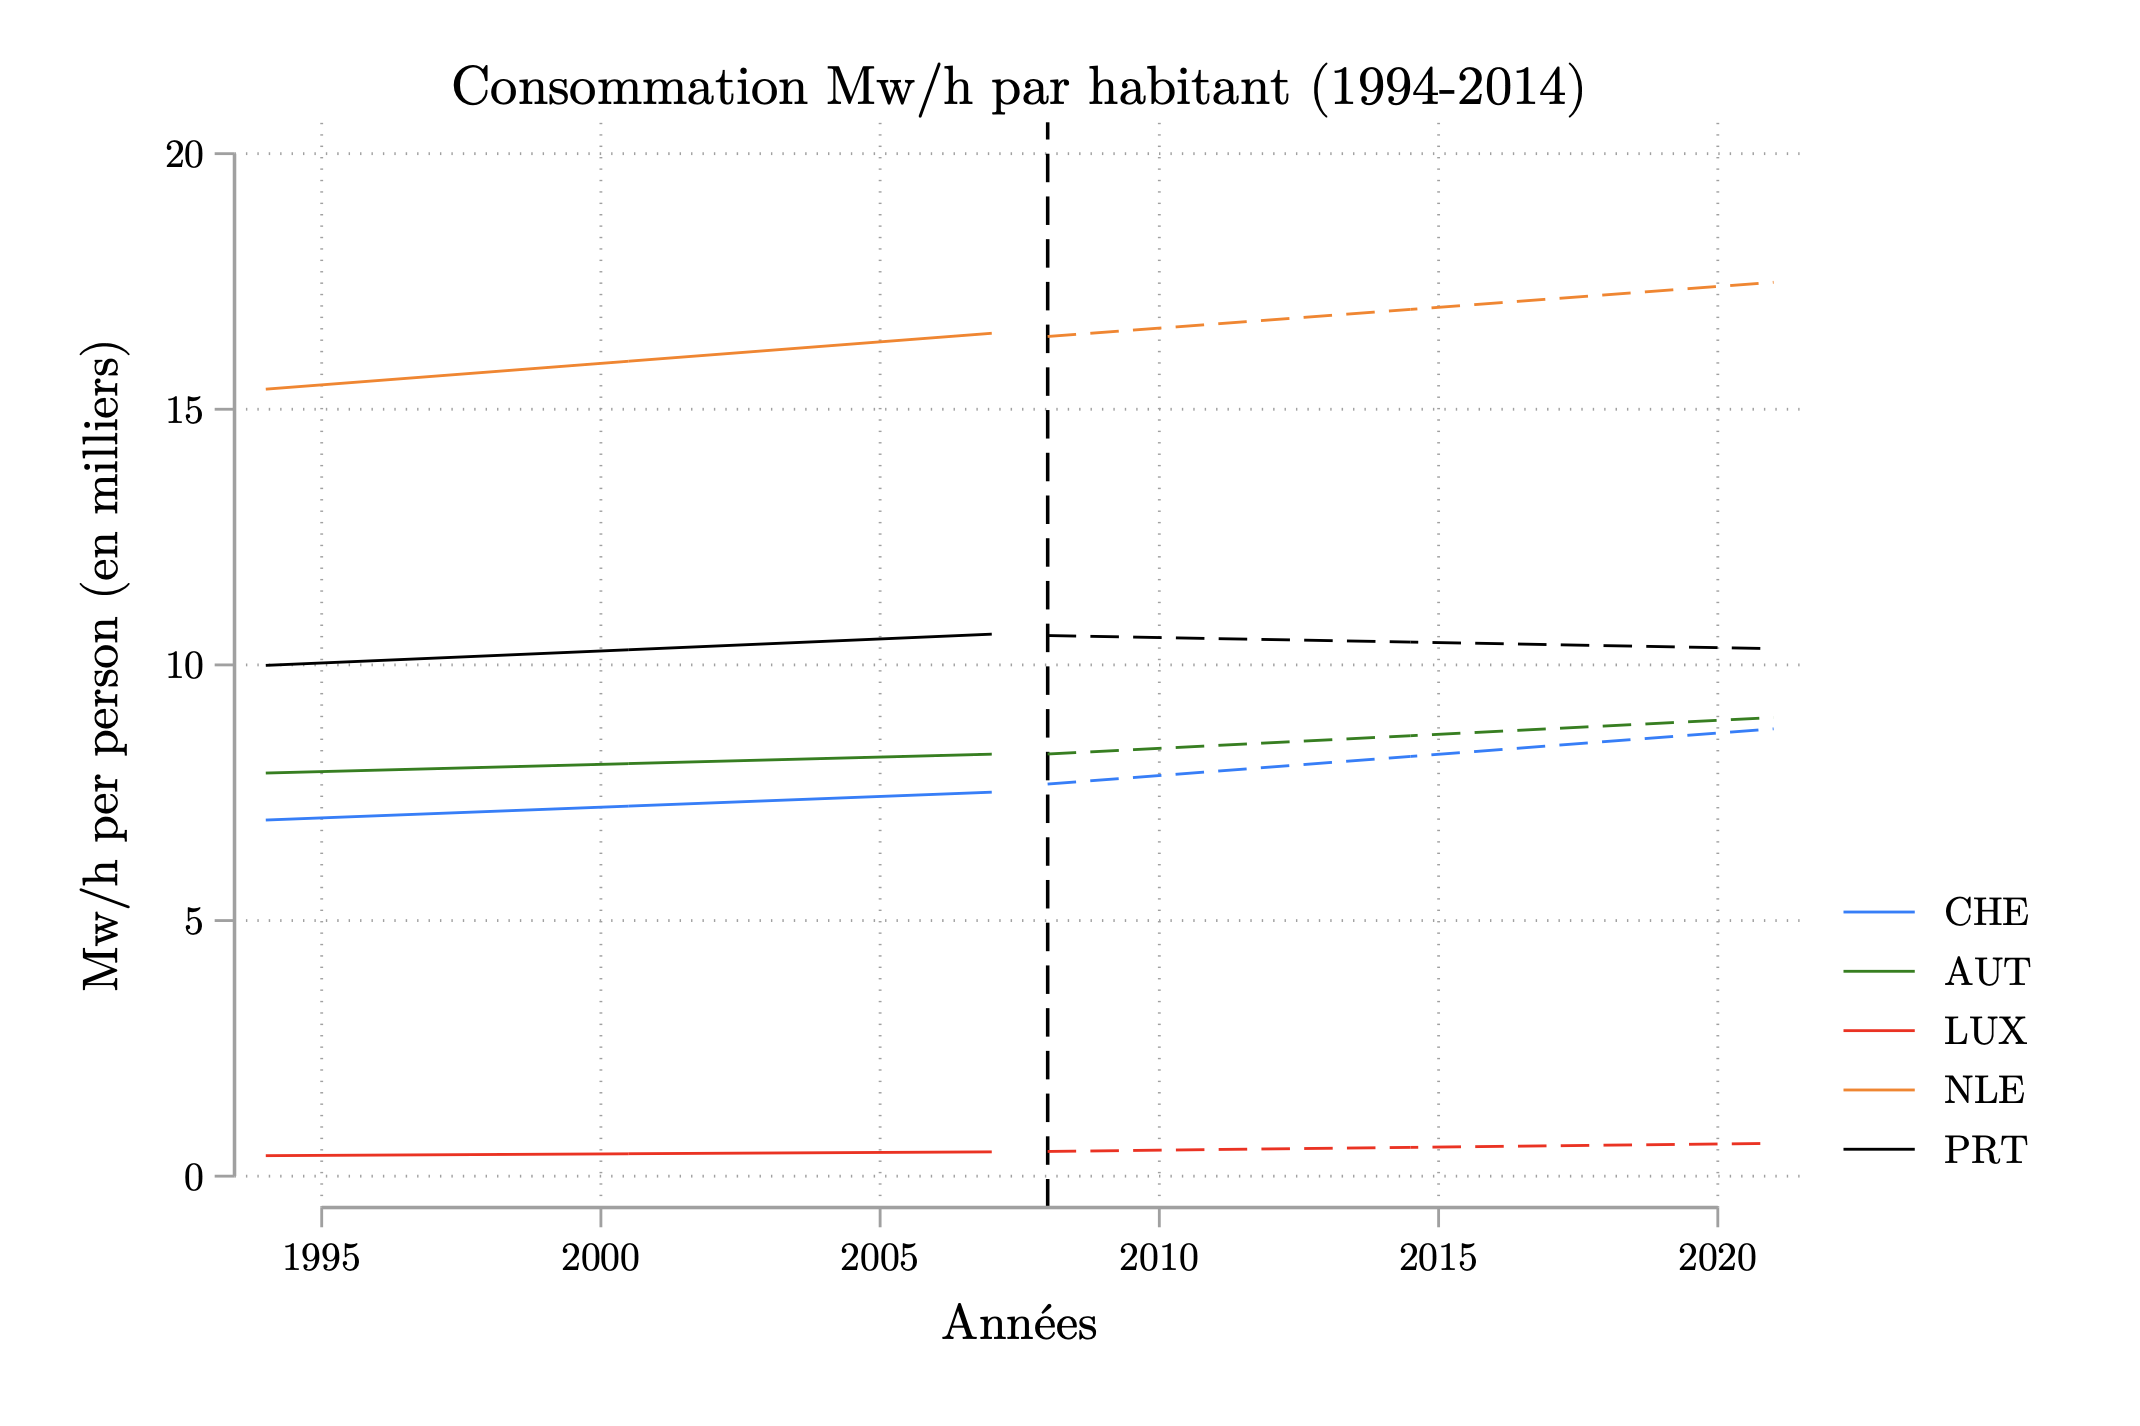
\includegraphics[width=0.6\textwidth]{Article/images/trend_electricite.png}
        \caption{}
        \label{fig:trend_megawats}
\begin{center}
Élimination : Portugal et Luxembourg (écarts significatifs dans la consommation d'électricité par habitant par rapport à la Suisse).
\end{center}
    \end{figure}

    


% \vspace{1cm}
% \newpage

\begin{figure}[H]
\textbf{Figure {$\ref{fig:trend_vehicules}$}} : Le graphique ci-dessous compare les variables "véhicules" entre la Suisse et les pays candidats. Les écarts significatifs observés pour certains pays ont conduit à leur élimination à cette étape.


\centering
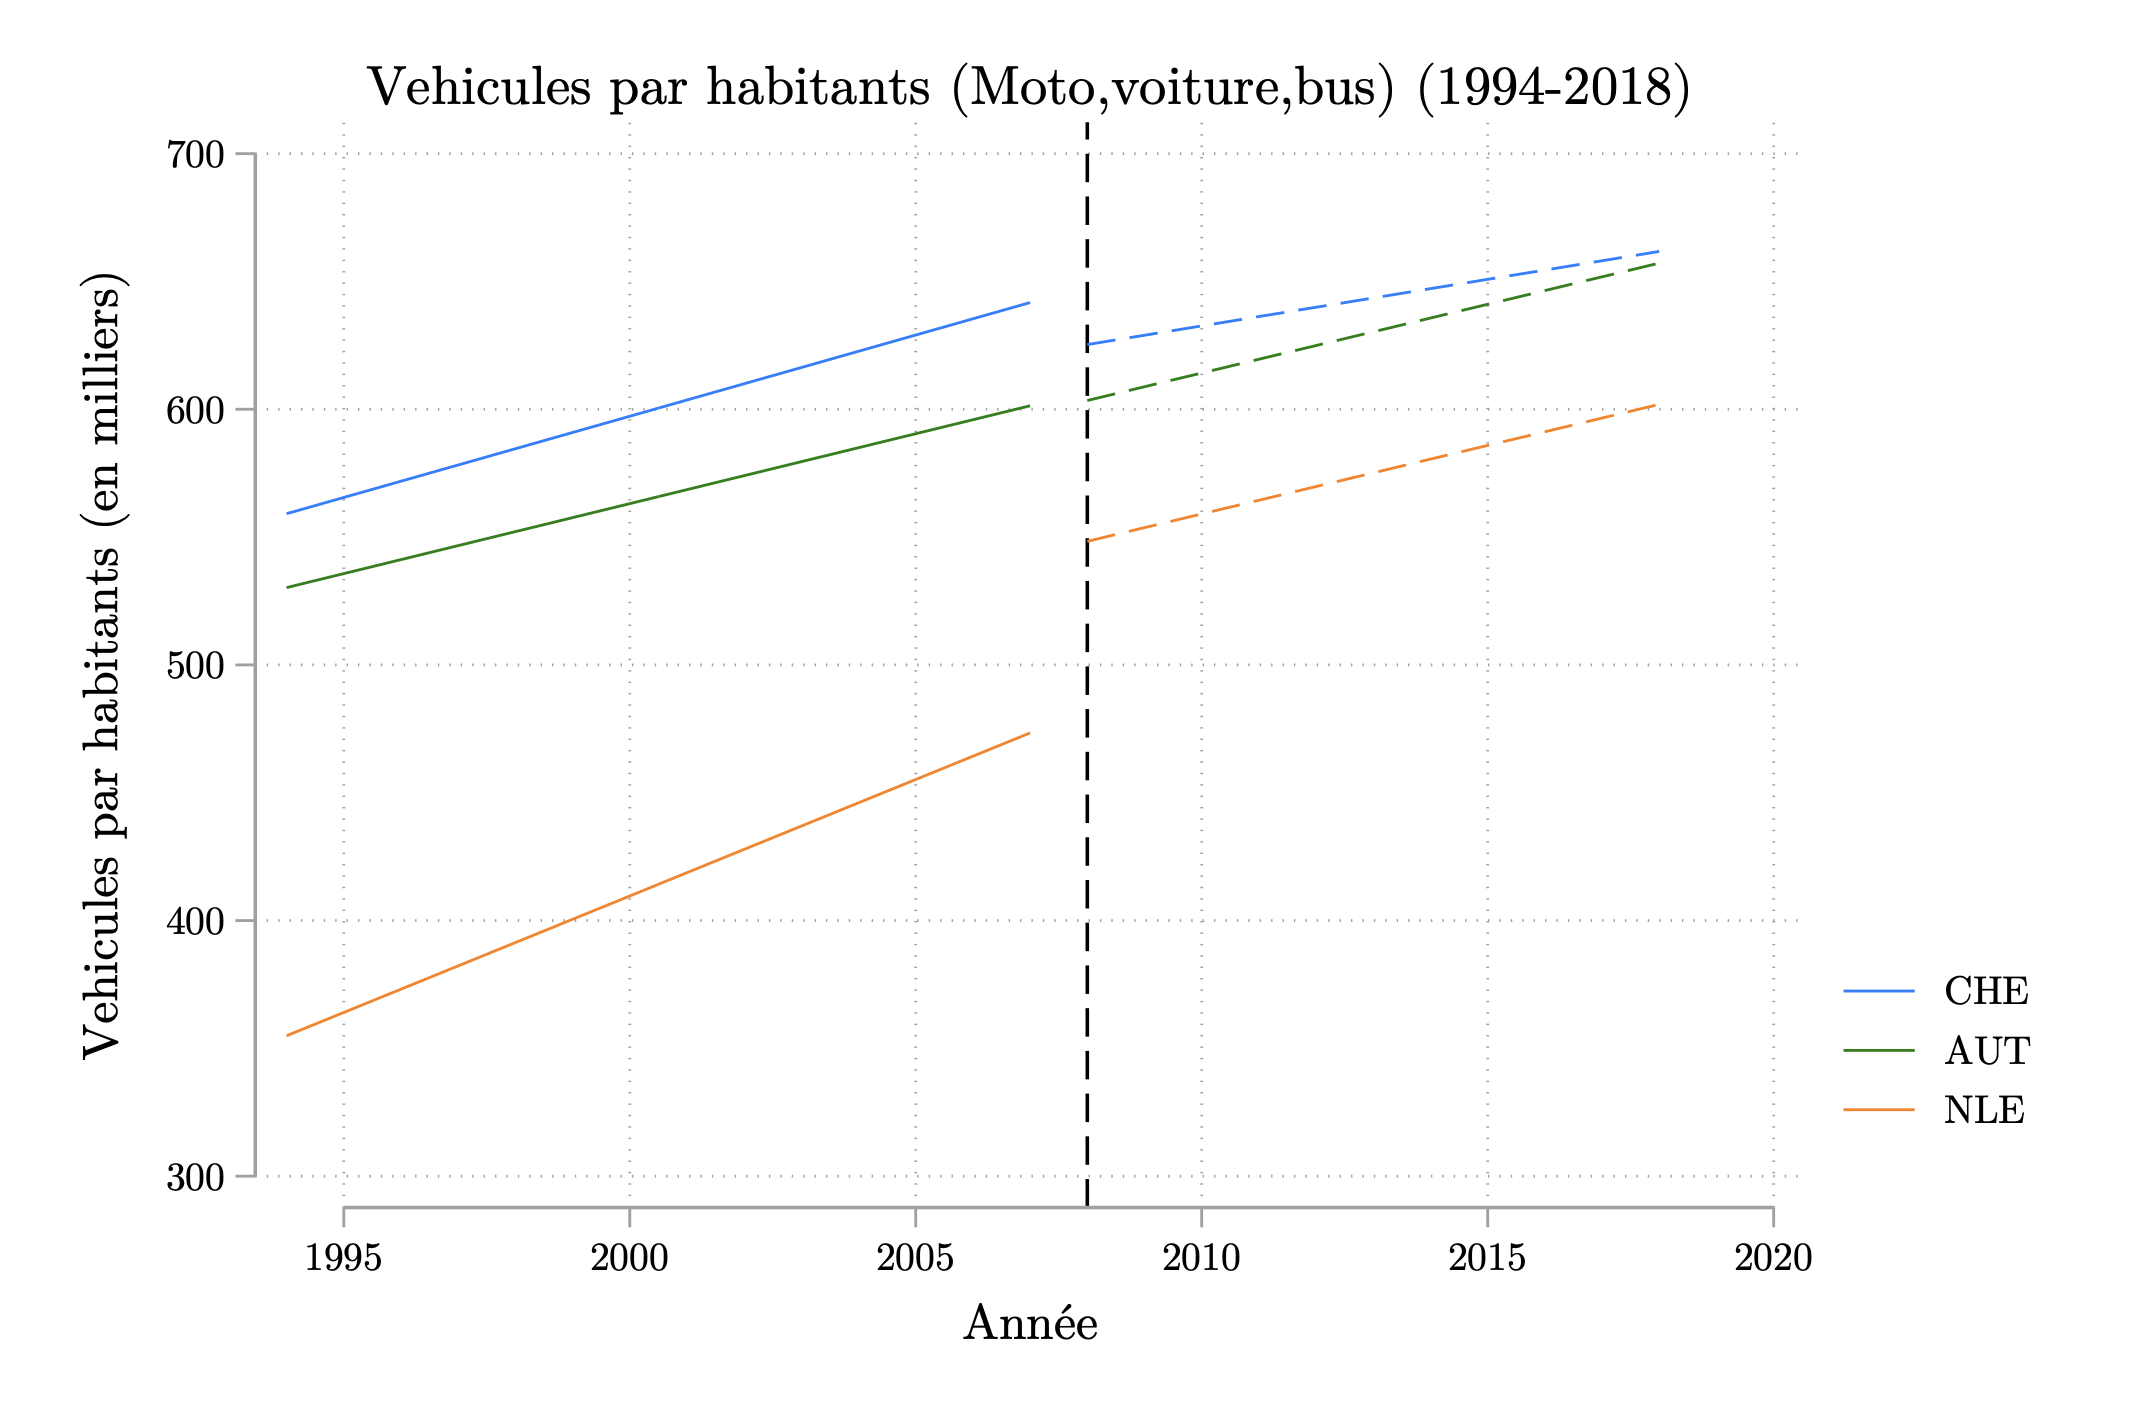
\includegraphics[width=0.6\textwidth]{Article/images/trend_vehicules.png}
\caption{}
\label{fig:trend_vehicules}
\begin{center}
    Élimination : Hollande (écart significatif du nombre de véhicules par rapport à la Suisse).
\end{center}
\end{figure}




Les graphiques montrent que l'Autriche présente les caractéristiques les plus similaires à celles de la Suisse avant l'introduction de la taxe, ce qui justifie sa sélection comme pays de contrôle optimal.

%------------------------------------------------------------------------------------%
\subsection{Tendances parallèles}
\label{subsec:pt}
%------------------------------------------------------------------------------------%

L'analyse des tendances parallèles est essentielle pour vérifier que les émissions de CO2 en Suisse et en Autriche évoluent de manière similaire avant l'introduction de la taxe.

Pour vérifier la validité de notre choix de l'Autriche comme pays de contrôle, dans un premier temps nous avons procédé à une analyse visuelle des tendances parallèles en comparant les droites de régression des émissions de CO2 par habitant avant et après l'introduction de la taxe CO2 en Suisse et en Autriche. Cette analyse, basée sur des ajustements de courbes réalisés avec Stata, inclut des régressions séparées pour les périodes pré- et post-introduction de la taxe.

Les graphiques ci-dessous illustrent les tendances parallèles des émissions de CO2 par habitant pour la Suisse et l'Autriche. Chaque graphique montre les régressions des émissions de CO2 avant et après l'introduction de la taxe CO2 (2008) en Suisse, en fonction du temps :



\begin{figure}[H]
\centering
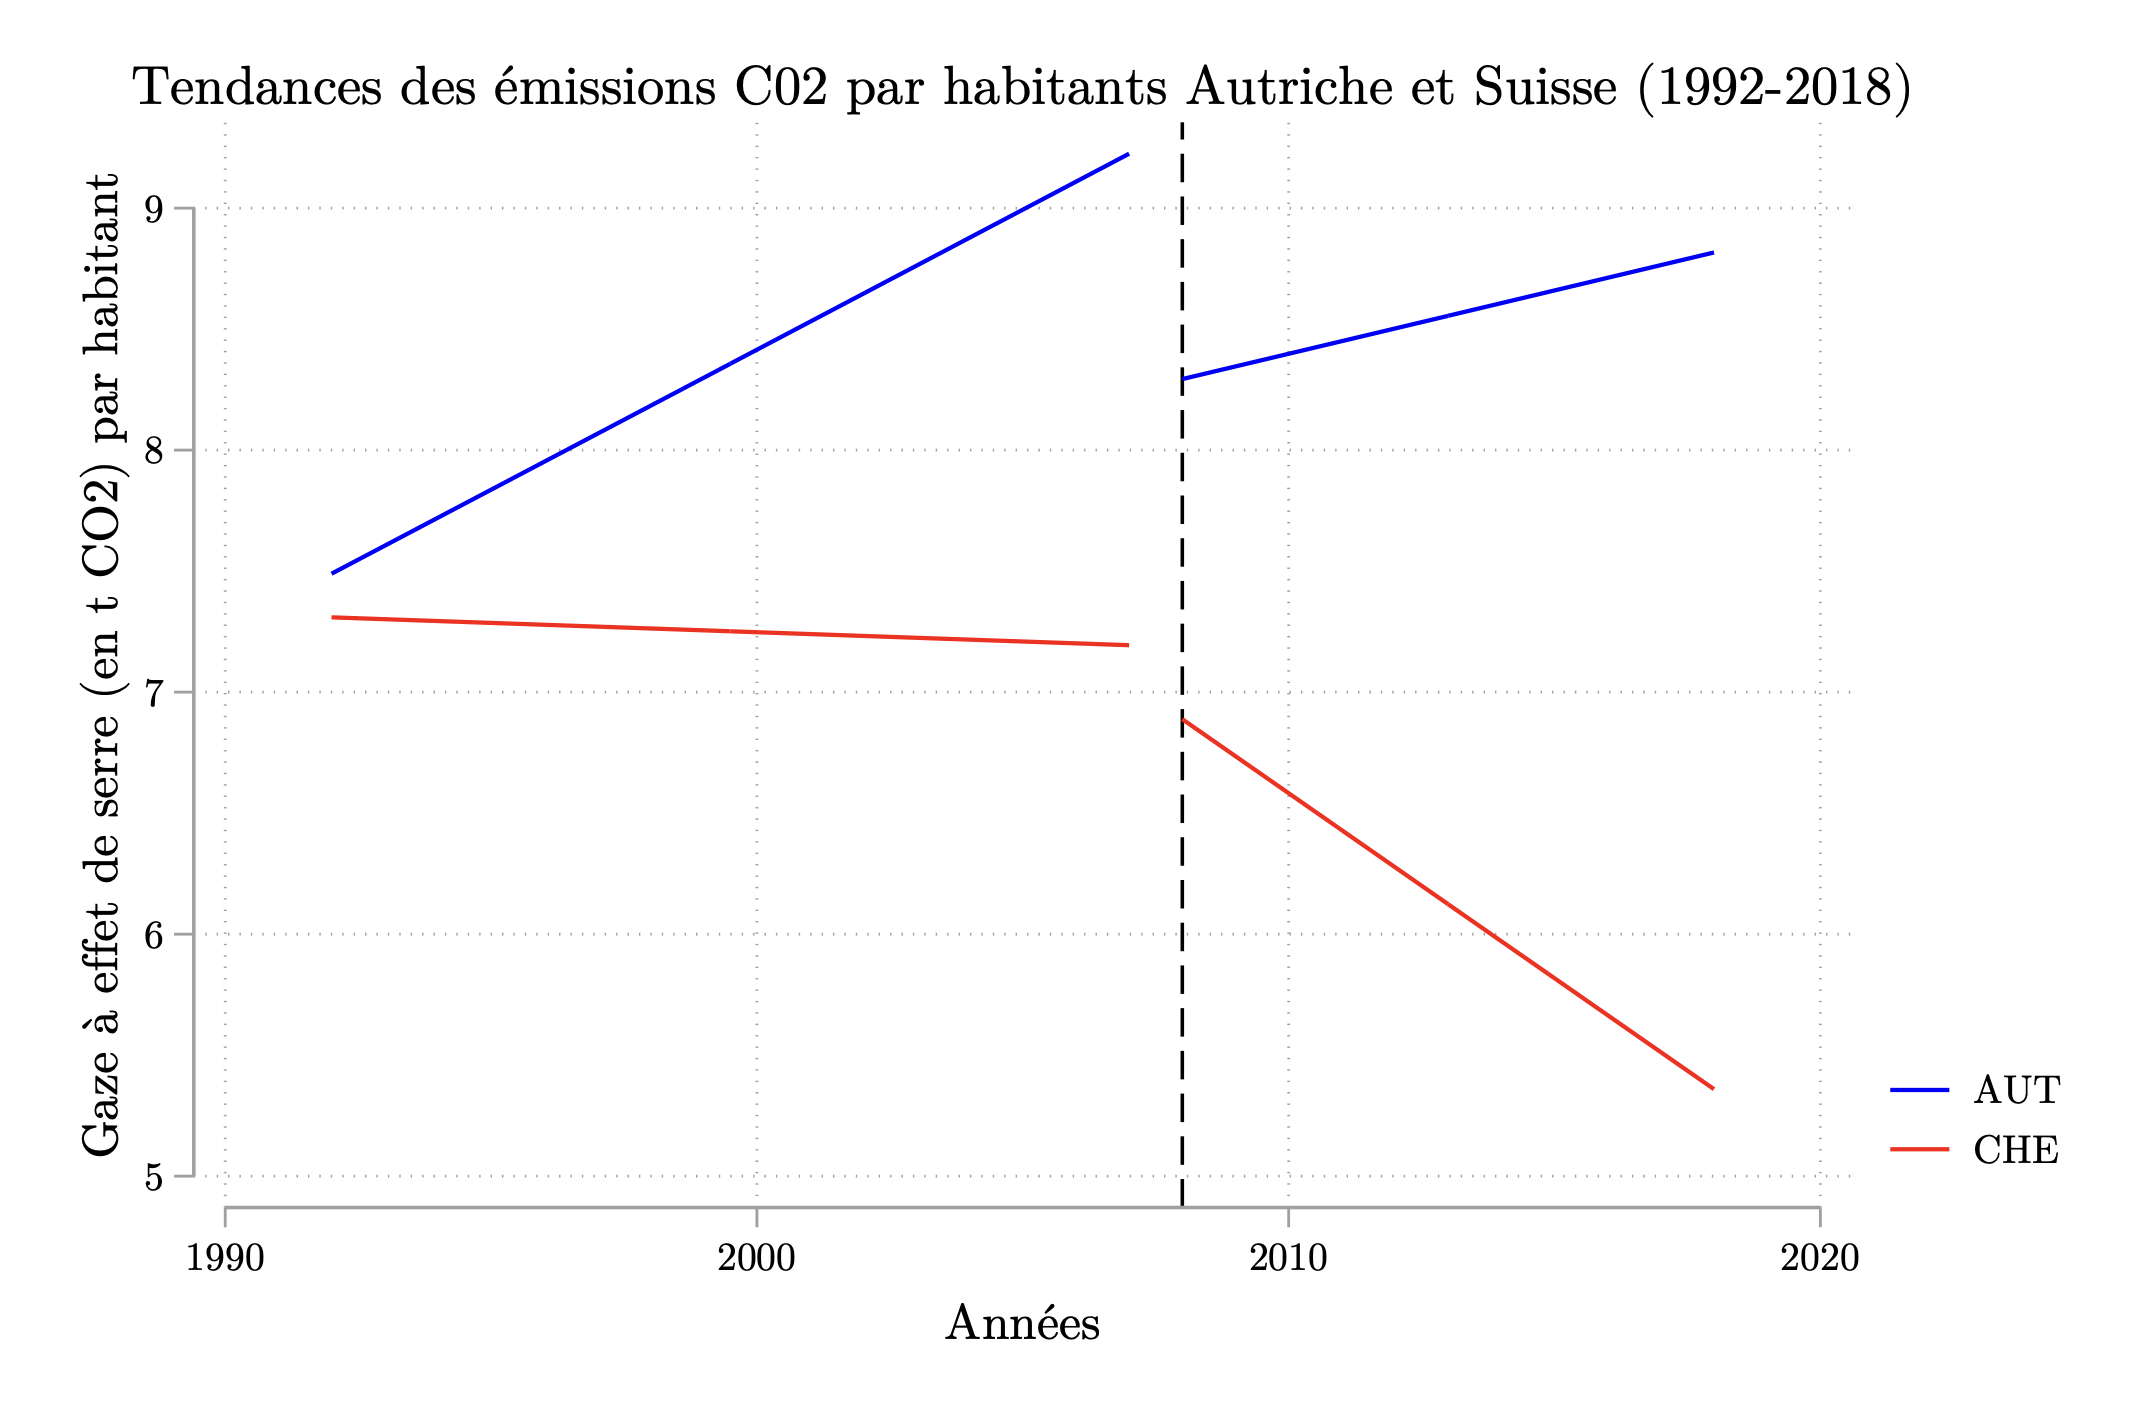
\includegraphics[width=0.7\textwidth]{Article/images/ptrend.png}
\caption{}
\label{fig:ptrend}
\end{figure}


Cette analyse a révélé que les tendances des émissions de CO2 en Suisse et en Autriche n'étaient pas parfaitement parallèles avant l'introduction de la taxe, mais ont divergé après, suggérant l'indice d'un effet causal potentiel de la taxe CO2 en Suisse. Ces résultats renforcent la validité de notre choix de l'Autriche comme pays de contrôle pour cette étude.


%------------------------------------------------------------------------------------%
\subsection{Statistiques descriptives}
\label{subsec:stat_descriptives}
%------------------------------------------------------------------------------------%



Les statistiques descriptives des variables clés pour la Suisse et l'Autriche sont présentées ci-dessous. Ces statistiques incluent les moyennes, les écarts-types, les valeurs minimales et maximales, ainsi que les mesures de skewness et kurtosis.

\textbf{Tableau 1} : Statistiques descriptives pour la Suisse


\begin{table}[H]
    \centering
\def\sym#1{\ifmmode^{#1}\else\(^{#1}\)\fi}
    \footnotesize{
\begin{tabular}{|l*{1}{|ccccccc|}}
\hline
            &       count&        mean&          sd&         min&         max&    skewness&    kurtosis\\
\hline
co2\_par\_habitant&          24&    6.726318&    .7065699&    5.362008&    8.226878&   -.3268356&    2.652837\\
population  &          24&     7624234&    498540.5&     6993795&     8514327&    .3961959&    1.786073\\
pib\_par\_habitant&          24&    1.016208&    1.548065&      -3.524&       3.533&   -.7269177&     4.39657\\
transport\_passager&          24&    16469.35&    3375.026&       11713&     20864.5&   -.1273545&    1.418265\\
vehicules   &          24&    619.1407&    31.21581&    558.8837&    660.2146&    -.620953&    2.209551\\
\hline
\(N\)       &          24&            &            &            &            &            &            \\
\hline
\end{tabular}
}
    \caption{Suisse}
    \label{tab:Suisse}
\end{table}


% \newpage 

\textbf{Tableau 2} : Statistiques descriptives pour l'Autriche


\begin{table}[H]
    \centering
\def\sym#1{\ifmmode^{#1}\else\(^{#1}\)\fi}
    \footnotesize{
\begin{tabular}{|l*{1}{|ccccccc|}}
\hline
            &       count&        mean&          sd&         min&         max&    skewness&    kurtosis\\
\hline
co2\_par\_habitant&          24&    8.473309&    .7676608&    6.849714&    9.848569&   -.0141597&    2.426966\\
population  &          24&     8278559&    284703.3&     7936118&     8837707&    .4853689&    2.121993\\
pib\_par\_habitant&          24&    1.423792&    1.649941&      -4.016&       3.468&   -1.418378&    5.937025\\
transport\_passager&          24&    10102.89&    1720.486&        7971&     13204.7&    .2656032&    1.719964\\
vehicules   &          24&    594.8536&    41.32612&    505.4989&    656.0979&   -.4380238&    2.406504\\
\hline
\(N\)       &          24&            &            &            &            &            &            \\
\hline
\end{tabular}
}
    \caption{Autriche}
    \label{tab:Autriche}
\end{table}


\vspace*{0.5cm}

\begin{itemize}[itemsep=-0.3em]
    \item[] \textbf{CO2 par habitant : }
    \item[] Les moyennes des émissions de CO2 par habitant sont plus élevées en Autriche (8.47) qu'en Suisse (6.73). Cette différence suggère que l'Autriche pourrait avoir des politiques environnementales moins strictes ou des sources d'énergie plus polluantes, ce qui pourrait influencer l'impact observé de la taxe CO2 en Suisse. Comprendre ces différences est crucial pour interpréter correctement les effets de la taxe dans le contexte de politiques et de structures énergétiques différentes.

    \item[] \textbf{Population : }
    \item[] La population des deux pays est relativement similaire, bien que l'Autriche ait une population légèrement plus élevée. Cette similitude démographique renforce la comparaison entre les deux pays pour l'analyse des émissions de CO2.

    \item[] \textbf{PIB par habitant : }
    \item[] Les PIB moyens par habitant indiquent une certaine prospérité économique dans les deux pays, avec des valeurs similaires mais une plus grande variabilité en Autriche. Cela montre que les deux pays ont des contextes économiques comparables, ce qui est favorable pour notre étude.

    \item[] \textbf{Transport passager :}
    \item[] La Suisse a une moyenne plus élevée de passagers par rail (16,469.35) comparée à l'Autriche (10,102.89), ce qui pourrait indiquer une infrastructure ferroviaire plus développée ou une plus grande utilisation des transports en commun en Suisse. Cette différence est importante à considérer dans notre analyse des émissions de CO2.

    \item[] \textbf{Véhicules : }
    \item[] Le nombre moyen de véhicules par habitant est légèrement supérieur en Suisse (619.14) qu'en Autriche (594.85). Cela suggère des différences dans l'utilisation des véhicules privés, ce qui peut influencer les émissions de CO2.

    \item[] \textbf{Skewness et kurtosis : }
    \item[] Les valeurs de skewness et kurtosis montrent que les distributions des variables sont relativement normales, ce qui est favorable pour les analyses statistiques ultérieures.
\end{itemize}

Les statistiques descriptives entre les tableaux$^{ \left[\ref{tab:Suisse}, \ref{tab:Autriche} \right]}$ montrent des différences mais aussi des similitudes importantes entre la Suisse et l'Autriche, renforçant la validité de notre choix de l'Autriche comme pays de contrôle pour étudier l'impact de la taxe CO2 en Suisse. Ces observations fournissent un contexte solide pour l'analyse économétrique qui suivra.



\subsubsection{Groupe de contrôle synthétique}
\label{subsubsec:control_synth}

En complément de l'analyse DiD, nous avons employé la méthode de contrôle synthétique (SCM) pour créer un groupe de contrôle synthétique, incluant principalement le Luxembourg et la Hollande. Le groupe de contrôle synthétique a été utilisé pour pallier les limitations de l'analyse DiD en offrant un point de comparaison composite plus robuste.

\textbf{Sélection et pondération des pays dans le groupe synthétique :} 
Le Luxembourg et la Hollande ont été choisis pour leurs similitudes avec la Suisse sur certaines variables clés. Les pondérations des pays ont été déterminées pour maximiser la similarité entre le groupe synthétique et la Suisse avant l'introduction de la taxe. Le Portugal a été exclu en raison de données manquantes pour les véhicules, ce qui aurait pu introduire des biais dans l'analyse.

\textbf{Table \ref{tab:Luxembourg}} : Statistiques descriptives pour le Luxembourg




    \footnotesize{
\begin{table}[H]
    \centering
\def\sym#1{\ifmmode^{#1}\else\(^{#1}\)\fi}
    \footnotesize{
\begin{tabular}{|l*{1}{|ccccccc|}}
\hline
            &       count&        mean&          sd&         min&         max&    skewness&    kurtosis\\
\hline
co2\_par\_habitant&          24&    21.78969&    3.369169&    16.46988&    29.79294&    .2476584&    2.750566\\
population  &          24&    487229.5&    63438.43&      402921&      607950&    .4468255&    1.969461\\
pib\_par\_habitant&          24&    1.579542&    2.975673&      -5.034&       6.962&     .173373&    2.749789\\
transport\_passager&          24&       338.5&     56.1837&         262&         442&    .4765047&    1.997054\\
vehicules   &          24&    502.8899&     68.7504&    384.8425&    598.8957&   -.3951171&    1.739076\\
\hline
\(N\)       &          24&            &            &            &            &            &            \\
\hline
\end{tabular}
    \caption{Luxembourg}
    \label{tab:Luxembourg}
\end{table}
}

% \newpage 

\textbf{Tableau \ref{tab:Hollande}} : \normalsize Statistiques descriptives pour la Hollande


\begin{table}[H]
    \centering
    \def\sym#1{\ifmmode^{#1}\else\(^{#1}\)\fi}
\footnotesize{
    \begin{tabular}{|l*{1}{|ccccccc|}}
        \hline
        & count & mean & sd & min & max & skewness & kurtosis \\
        \hline
        co2\_par\_habitant & 24 & 13.32603 & 1.455271 & 11.08089 & 15.94756 & .2042466 & 1.893743 \\
        population & 24 & 1.63e+07 & 553078.9 & 1.54e+07 & 1.72e+07 & -.1708392 & 1.91928 \\
        pib\_par\_habitant & 24 & 1.592958 & 1.94239 & -4.107 & 4.435 & -1.043792 & 4.321272 \\
        transport\_passager & 24 & 15624.08 & 1959.168 & 12800 & 22600 & 1.762031 & 7.920342 \\
        vehicules & 24 & 487.2914 & 89.23535 & 363.5235 & 604.0096 & -.0539008 & 1.271187 \\
        \hline
        \(N\) & 24 & & & & & & \\
        \hline
    \end{tabular}
}
    \caption{Hollande}
    \label{tab:Hollande}
\end{table}

\normalsize

Les statistiques descriptives entre les tableaux $^{ \left[\ref{tab:Suisse}, \ref{tab:Luxembourg}, \ref{tab:Hollande} \right]}$ révèlent des différences et des similitudes entre la Suisse, l'Autriche et la Hollande. L'Autriche présente des niveaux de CO2 par habitant plus élevés, tandis que la Hollande a des niveaux intermédiaires. Les populations et les PIB par habitant montrent des différences, ce qui est crucial pour comprendre les dynamiques économiques et démographiques qui peuvent influencer les émissions de CO2. Le transport passager par rail est beaucoup plus élevé en Suisse et en Hollande, ce qui peut jouer un rôle dans les différences d'émissions de CO2 observées. Ces observations fournissent un contexte solide pour l'analyse économétrique qui suivra, justifiant l'utilisation de l'Autriche, la Hollande et du Luxembourg dans la construction du groupe de contrôle synthétique, malgré les différences observées. Ces pays ont été sélectionnés comme les meilleurs candidats disponibles - en fonction des données disponibles - pour créer un groupe de contrôle robuste.










